\subsection{Similarity-stratified test analysis}
To assess how chemical novelty relates to test performance, each scaffold-test molecule was assigned the maximum Morgan-fingerprint Tanimoto similarity to any scaffold-training molecule. Four empirical quantile bins were constructed from similarity alone before model labels or predictions were inspected. Duplicate quantile cut points were collapsed, keeping equal-similarity molecules together. Within each bin, ROC AUC and PR AUC were calculated separately for each endpoint using only observed labels. Endpoint scores were averaged within seed, then summarized across the three model seeds. No model or hyperparameter was selected using this analysis.

The mean endpoint PR AUC is higher in the most similar bin than in the least similar bin for XGBoost (0.588 vs. 0.308), the graph MPNN (0.477 vs. 0.260), and H1 (MPNN with descriptors; 0.582 vs. 0.257). The pattern is not strictly monotonic: both XGBoost and the graph MPNN dip in the second bin. The comparison is descriptive and does not establish that similarity causes the performance difference. The four bins contain 191--195 molecules each, while the number of observed labels varies across endpoints.

\begin{table*}[t]
\centering
\caption{Scaffold-test performance by maximum Tanimoto similarity to the training set. PR AUC is averaged across endpoints within seed; uncertainty is the sample SD across three model seeds.}
\label{tab:tanimoto-binned}
\begin{tabular}{llrrr}
\toprule
Model & Similarity quantile & Molecules & Mean PR AUC & Seed SD \\
\midrule
XGBoost & Q1 [0.143, 0.308] & 195 & 0.308 & 0.015 \\
XGBoost & Q2 [0.308, 0.396] & 191 & 0.266 & 0.005 \\
XGBoost & Q3 [0.396, 0.524] & 192 & 0.467 & 0.008 \\
XGBoost & Q4 [0.524, 1.000] & 193 & 0.588 & 0.006 \\
MPNN & Q1 [0.143, 0.308] & 195 & 0.260 & 0.046 \\
MPNN & Q2 [0.308, 0.396] & 191 & 0.215 & 0.023 \\
MPNN & Q3 [0.396, 0.524] & 192 & 0.383 & 0.015 \\
MPNN & Q4 [0.524, 1.000] & 193 & 0.477 & 0.040 \\
H1 (MPNN + desc.) & Q1 [0.143, 0.308] & 195 & 0.257 & 0.011 \\
H1 (MPNN + desc.) & Q2 [0.308, 0.396] & 191 & 0.269 & 0.013 \\
H1 (MPNN + desc.) & Q3 [0.396, 0.524] & 192 & 0.426 & 0.019 \\
H1 (MPNN + desc.) & Q4 [0.524, 1.000] & 193 & 0.582 & 0.031 \\
\bottomrule
\end{tabular}
\end{table*}


\begin{figure}[t]
    \centering
    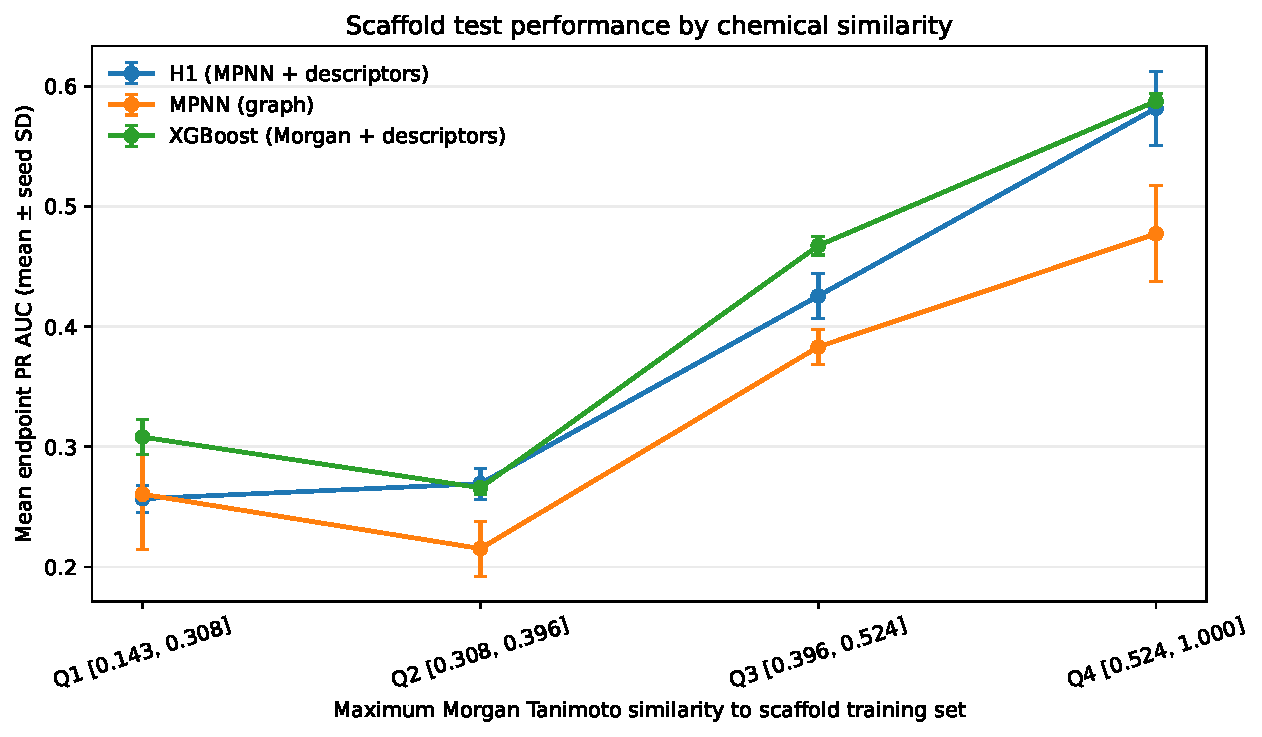
\includegraphics[width=\linewidth]{figures/tanimoto.pdf}
    \caption{Mean endpoint PR AUC by maximum Morgan Tanimoto similarity to the scaffold training set. Error bars show sample SD across three model seeds.}
    \label{fig:phase2-tanimoto}
\end{figure}

\subsection{Architecture ablations and shuffled-label control}
All ablations use the frozen MPNN configuration in \texttt{results/best\_configs\_dl.json} (hidden size 64, three message-passing steps, dropout 0.2, learning rate $10^{-3}$, and weight decay $10^{-5}$) on the scaffold split with seeds 0--2. The predeclared comparisons change one property at a time: message-passing depth, bond features, or graph readout. Each seed's metric is the mean over the 12 endpoints; the table reports the mean and sample standard deviation of those three seed-level means. All values are computed from \texttt{results/dl\_ablation\_test\_malhar.csv}.

\begin{table*}[t]
\centering
\caption{Malhar's MPNN architecture ablations on the scaffold test split. Values are mean endpoint AUC $\pm$ sample SD across seeds 0--2, computed from the committed ablation CSV.}
\label{tab:member5-ablation}
\small
\begin{tabular}{lcc}
\toprule
Variant & PR AUC & ROC AUC \\
\midrule
A1: depth 1 & $0.2846 \pm 0.0129$ & $0.7388 \pm 0.0107$ \\
A2: depth 2 & $0.3007 \pm 0.0071$ & $0.7353 \pm 0.0096$ \\
A3: no bonds & $0.2947 \pm 0.0437$ & $0.7439 \pm 0.0187$ \\
P2: depth 4 & $0.2818 \pm 0.0172$ & $0.7311 \pm 0.0153$ \\
P2: sum readout & $0.3125 \pm 0.0172$ & $0.7586 \pm 0.0156$ \\
P2: mean readout & $0.3001 \pm 0.0043$ & $0.7391 \pm 0.0019$ \\
C1: shuffled labels & $0.1382 \pm 0.0063$ & $0.5305 \pm 0.0302$ \\
\bottomrule
\end{tabular}
\end{table*}

The shuffled-label control permutes complete training-label rows across molecules and leaves validation and test labels unchanged. Its three seed-level mean test ROC AUCs are 0.5038, 0.5246, and 0.5632. Although the three-seed mean is 0.5305, seed 2 exceeds the predeclared 0.55 threshold. This is a warning that warrants a leakage investigation; averaging across seeds does not remove it.

\subsection{Prediction alignment and seed variability}
The saved probability arrays were checked against their split's test-label order and corresponding result CSVs. Every available file had shape $771\times12$, contained finite probabilities in $[0,1]$, and reproduced all per-endpoint label counts, ROC AUCs, and PR AUCs within $2\times10^{-6}$. The audit covers XGBoost and graph MPNN on both splits and H1 on the scaffold split. Seed variability is calculated after averaging over endpoints, so it reflects model randomness on one fixed split rather than split-to-split uncertainty.

\begin{table}[t]
\centering
\caption{Test-set performance and model-seed variability. Values are endpoint means with sample SD across the three model seeds.}
\label{tab:member5-seed-variance}
\begin{tabular}{llrr}
\hline
Model & Split & ROC AUC & PR AUC \\
\hline
MPNN (graph) & random & 0.815 $\pm$ 0.015 & 0.439 $\pm$ 0.041 \\
XGBoost (Morgan + descriptors) & random & 0.862 $\pm$ 0.002 & 0.565 $\pm$ 0.002 \\
MPNN (graph) & scaffold & 0.729 $\pm$ 0.014 & 0.307 $\pm$ 0.018 \\
H1 (MPNN + descriptors) & scaffold & 0.738 $\pm$ 0.007 & 0.355 $\pm$ 0.006 \\
XGBoost (Morgan + descriptors) & scaffold & 0.761 $\pm$ 0.004 & 0.401 $\pm$ 0.005 \\
\hline
\end{tabular}
\end{table}

